\section{Auswertung}
\label{sec:auswertung}

\subsection{Stabilitätsbedingung}
\label{sec:auswertung:stabilitaetsbedingung}
% Aufgabe 2 in der Versuchsanleitung

In \autoref{sec:stabilitaet} wurde anhand der \hyperref[eqn:stabilitaetsbedingung]{Stabilitätsbedingung} die maximale theoretische Resonatorlänge berechnet.
Um diese experimentell zu überprüfen,
wird die Intensität des Lasers für verschiedene Resonatorlängen und Spiegelkonfigurationen gemessen.
\autoref{fig:plt:stabilitaetsbedingung} stellt diese Messwerte dar; die zugrundeliegenden Daten sind in \autoref{tab:stabilitaetsbedingung} aufgeführt.
% In \autoref{fig:plt:stabilitaetsbedingung} sind diese Messwerte dargestellt.

Es ist zu beachten, dass diejenigen Resonatorlängen, bei denen kein Lasern einsetzte, nicht angegeben sind.
Andererseits waren aufgrund der begrenzten Länge der optischen Bank keine größeren Resonatorlängen als etwa \SI{212.8}{\centi\meter} möglich.

\begin{figure}
  \centering
   \includegraphics[width=\textwidth]{build/plt/2_stabilitaetsbedingung.pdf}
   \caption{Lichtintensität $I$ in Abhängigkeit der Resonatorlänge $L$ für verschiedene Spiegelkonfigurationen.}
   \label{fig:plt:stabilitaetsbedingung}
\end{figure}

\begin{table}
\centering
\caption{Messwerte zur Lichtintensität $I$ in Abhängigkeit der Resonatorlänge $L$ für verschiedene Spiegelkonfigurationen.}
\label{tab:stabilitaetsbedingung}
\begin{subtable}{.5\textwidth}
    \centering
    \caption{\enquote{konkav + konkav}}
    \expandableinput{build/tab/2_stabilitaetsbedingung_konkav_konkav.tex}
\end{subtable}%
\begin{subtable}{.5\textwidth}
    \centering
    \caption{\enquote{plan + konkav}}
    \expandableinput{build/tab/2_stabilitaetsbedingung_plan_konkav.tex}
\end{subtable}
\end{table}


% TODO: Mit Theorie-Abschnitt vereinigen
% Durch Lösen von \autoref{eqn:TODO} können die theoretisch größtmöglichen Resonatorlängen $L$ bestimmt werden.
% Hierbei ist zu beachten, dass bei Gleichheit nur noch ein metastabiler Zustand vorliegt.
% \begin{align*}
%     L_\text{max, kk, theo} &= r_1 + r_2 \\
%     L_\text{max, pk, theo} &= r_2 \\
% \end{align*}


\subsection{TEM-Moden}
\label{sec:auswertung:tem_moden}
% Aufgabe TODO in der Versuchsanleitung

\subsubsection{\TEM{00}-Mode}
Die Lichtintensität der \TEM{00}-Mode wird (bei Betrachtung senkrecht zur Strahlachse) durch eine Gauß-Funktion beschrieben.
Um die gemessene Intensitätsverteilung sinnvoll mit der theoretischen zu vergleichen,
werden dabei zusätzliche Parameter für Hintergrund und Verschiebung der Strahlachse eingesetzt.
Daraus ergibt sich \autoref{eqn:tem00_fitfn},
deren Parameter mithilfe von \scipycurvefit an die Messwerte angepasst werden.
\autoref{fig:plt:tem_00} stellt Messwerte und Theoriekurve grafisch dar;
die zugrundeliegenden Daten sind in \autoref{tab:mess_tem_00} aufgeführt.

\begin{equation}
  I =
  I_\text{max} \cdot \exp \left( \frac{-(r - r_0)^2}{2ω^2} \right) + I_0
  \label{eqn:tem00_fitfn}
\end{equation}


Es ergeben sich die folgenden Parameter:
\begin{align*}
  I_\text{max} &= \SI{131.5 \pm 1.1}{\micro\watt}
  \tag{maximale Intensität}
  \\
  I_0 &= \SI{1.7 \pm 0.5}{\micro\watt}
  \tag{Hintergrund, beispielsweise durch Streulicht}
  \\
  r_0 &= \SI{0.082 \pm 0.018}{\milli\meter}
  \tag{Mittelpunkt des Laserstrahls} % bzw. Verschiebung von Strahlachse
  \\
  ω &= \SI{1.968 \pm 0.021}{\milli\meter} % Vorzeichen ist irrelevant!
  \tag{Breite der Gauß-Verteilung}
  \\
\end{align*}

\begin{figure}
  \centering
   \includegraphics[width=\textwidth]{build/plt/3_tem_00.pdf}
   \caption{Lichtintensität $I$ in Abhängigkeit der Distanz $r$ zur optischen Achse für die \TEM{00}-Mode.}
   \label{fig:plt:tem_00}
\end{figure}


\subsubsection{\TEM{01}-Mode}
Die Lichtintensität der \TEM{01}-Mode wird (bei Betrachtung senkrecht zur Strahlachse) durch \autoref{eqn:tem01_fitfn} beschrieben,
wenn wie zuvor zusätzliche Parameter für Hintergrund und Verschiebung der Strahlachse eingesetzt werden.
Das Anpassen der Parameter an die Messwerte erfolgt erneut mit \scipycurvefit.
\autoref{fig:plt:tem_01} stellt Messwerte und Theoriekurve grafisch dar;
die zugrundeliegenden Daten sind in \autoref{tab:mess_tem_01} aufgeführt.

\begin{equation}
  I =
  I_\text{max} \cdot
  \frac{4(r - r_0)^2}{ω^2} \cdot
  \exp \left( \frac{-(r - r_0)^2}{2ω^2} \right) + I_0
  \label{eqn:tem01_fitfn}
\end{equation}

Es ergeben sich die folgenden Parameter:
\begin{align*}
  I_\text{max} &= \SI{3.10 \pm 0.08}{\micro\watt}
  \tag{maximale Intensität}
  \\
  I_0 &= \SI{1.13 \pm 0.09}{\micro\watt}
  \tag{Hintergrund, beispielsweise durch Streulicht}
  \\
  r_0 &= \SI{0.304 \pm 0.024}{\milli\meter}
  \tag{Mittelpunkt des Laserstrahls} % bzw. Verschiebung von Strahlachse
  \\
  ω &= \SI{1.141 \pm 0.017}{\milli\meter} % Vorzeichen ist irrelevant!
  \tag{Breite der Gauß-Verteilung}
  \\
\end{align*}

\begin{figure}
  \centering
   \includegraphics[width=\textwidth]{build/plt/3_tem_01.pdf}
   \caption{Lichtintensität $I$ in Abhängigkeit der Distanz $r$ zur optischen Achse für die \TEM{01}-Mode.}
   \label{fig:plt:tem_01}
\end{figure}

% --- für TEM00 und TEM01 ↓
\begin{table}[H]
\centering
\caption{Messwerte zur Lichtintensität in Abhängigkeit der Distanz zur optischen Achse für verschiedene \TEM{}-Moden.}
\label{tab:mess_tem}
\begin{subtable}{.5\textwidth}
    \centering
    \caption{\TEM{00}}
    \label{tab:mess_tem_00}
    \expandableinput{build/tab/3_tem_00.tex}
\end{subtable}%
\begin{subtable}{.5\textwidth}
    \centering
    \caption{\TEM{01}}
    \label{tab:mess_tem_01}
    \expandableinput{build/tab/3_tem_01.tex}
\end{subtable}
\end{table}


\subsection{Polarisation}
\lipsum[1]

\begin{figure}
  \centering
   \includegraphics[width=\textwidth]{build/plt/4_polarisation.pdf}
   \caption{Lichtintensität $I$ in Abhängigkeit der Winkeleinstellung $\alpha$ des Polarisationsfilters.}
   \label{fig:plt:polarisation}
\end{figure}


\subsection{Multimodenbetrieb und Frequenzspektrum des Lasers}
% \subsection{Longitudinale Moden}
% 5. Multimodenbetrieb und Frequenzspektrum des Lasers
Für $L = \SI{162.9}{\centi\meter}$ wird mithilfe eines Oszilloskops das Frequenzspektrum des Lasers im Multimodenbetrieb ausgemessen,
wie in \autoref{fig:screenshot_oszilloskop} gezeigt.
Die Peaks sind in \autoref{tab:mess_frequenzspektrum} angegeben.

\begin{figure}
  \centering
   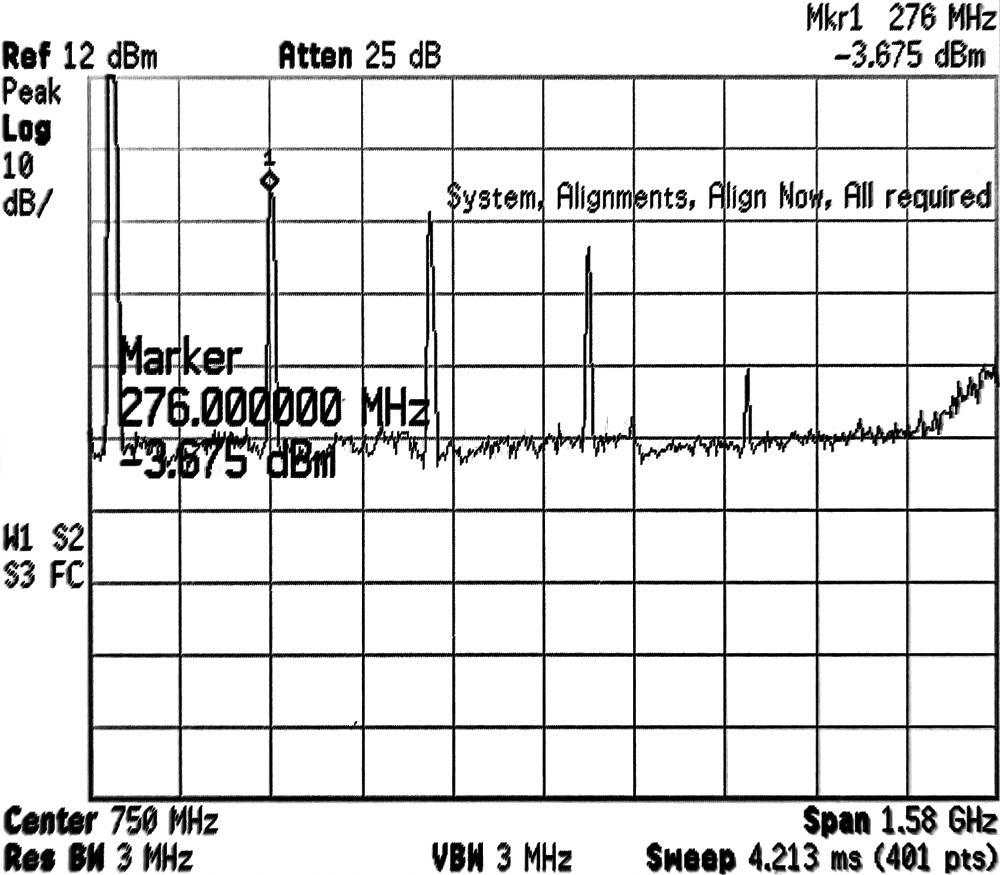
\includegraphics[width=0.75\textwidth]{content/img/5_frequenzspektrum_oszilloskop_inverted.jpg}
   \caption{Bildschirmfoto des Oszilloskops.}
   \label{fig:screenshot_oszilloskop}
\end{figure}

\begin{table}
  \centering
  \caption{Messwerte zur [TODO].}
  \label{tab:mess_frequenzspektrum}
  \begin{tabular}{S S}
  \toprule
  {$f \mathbin{/} \si{\mega\hertz}$} &
  {$I \mathbin{/} \si{dBm}$} \\ % Decibelmilliwatt
  \midrule
  276 & -3.4 \\
  553 & -7.1 \\
  829 & -12 \\
  1106 & -29 \\
  \bottomrule
  \end{tabular}
\end{table}



\subsection{Wellenlänge}
\label{sec:auswertung:wellenlaenge}
Um die Wellenlänge des Laserlichts zu bestimmen,
werden dessen Beugungsmaxima an verschiedenen optischen Gittern vermessen.

Durch Umformen von
\begin{equation*}
  k \lambda = d \sin(\alpha_k)
\end{equation*}
ergibt sich die praktisch anwendbare Bestimmungsgleichung
\begin{equation}
  \lambda = \frac{d a_k}{k \sqrt{e^2 + a_k^2}} \ ,
  \label{eqn:wellenlaenge}
\end{equation}
wobei $k$ die Ordnung des Beugungsmaximums,
$d$ der Spaltabstand (Gitterkonstante),
$e$ der Abstand zwischen Gitter und Schirm, % Oxford-Komma: Persönliche Präferenz, eigentlich nicht richtig.
und $a_k$ der Abstand des Beugungsmaximums zum Hauptmaximum (und somit zur optischen Achse)
ist.

Die Messwerte, anhand derer die Wellenlänge nun bestimmt wird, sind in \autoref{tab:mess_wellenlaenge} zu finden.
Dort sind auch die nach \autoref{eqn:wellenlaenge} bestimmten Wellenlängen für jede Messreihe angegeben.
Im Mittel ergibt sich $\bar\lambda = \SI{12345}{\micro\meter}$.

% Die Ordnung $k$ ist natürlich nicht wirklich vorzeichenbehaftet.
% TODO: In der Tabelle Vorzeichen streichen?

\begin{table}
  \centering
  \caption{
    Abstände der Interferenzmaxima der Ordnung $k$ vom Hauptmaximum für verschiedene optische Gitter.
    Zusätzlich sind die inverse Gitterkonstante $\sfrac{1}{d}$, der Abstand zum Schirm $e$ und die jeweils berechnete Wellenlänge $\lambda$ angegeben.
  }
  \label{tab:mess_wellenlaenge}
  \begin{tabular}{S S S S S}
  \toprule
  & \multicolumn{4}{c}{$\sfrac{1}{d} \mathbin{/} \si{\per\milli\meter}$} \\
  \cmidrule(lr){2-5}
  & 80 & 100 & 600 & 1200 \\
  \midrule

  & \multicolumn{4}{c}{$e \mathbin{/} \si{\centi\meter}$} \\
  \cmidrule(lr){2-5}
  & 90.5 & 90.5 & 63.0 & 33.0 \\
  \midrule

  {$k$} &
  \multicolumn{4}{c}{$a_k \mathbin{/} \si{\centi\meter}$} \\
  \midrule

  \expandableinput{build/tab/6_wellenlaenge.tex}
  \midrule

  & \multicolumn{4}{c}{$\lambda \mathbin{/} \si{\nano\meter}$} \\
  \cmidrule(lr){2-5}
  & 460.05 \pm 5.46 & 643.74 \pm 7.53 & 641.60 \pm 7.96 & 328.51 \pm 16.07 \\
  \bottomrule
  \end{tabular}
\end{table}
